\documentclass[a4j]{jarticle}

\usepackage[dvipdfmx]{graphicx}
\usepackage{url}
\usepackage{listings,jlisting}
\usepackage{ascmac}
\usepackage{amsmath,amssymb}

%ここからソースコードの表示に関する設定
\lstset{
  basicstyle={\ttfamily},
  identifierstyle={\small},
  commentstyle={\smallitshape},
  keywordstyle={\small\bfseries},
  ndkeywordstyle={\small},
  stringstyle={\small\ttfamily},
  frame={tb},
  breaklines=true,
  columns=[l]{fullflexible},
  numbers=left,
  xrightmargin=0zw,
  xleftmargin=3zw,
  numberstyle={\scriptsize},
  stepnumber=1,
  numbersep=1zw,
  lineskip=-0.5ex
}
%ここまでソースコードの表示に関する設定

\title{知能プログラミング演習II 課題3}
\author{グループ07\\
  29114095 野竹浩二朗\\
%  {\small (グループレポートの場合は、グループ名および全員の学生番号と氏名が必要)}
}
\date{2019年10月28日}

\begin{document}
\maketitle

\paragraph{提出物} rep3
\paragraph{グループ} グループ07
\paragraph{メンバー}
\begin{tabular}{|c|c|c|}
  \hline\hline
  学籍番号&名前&貢献度\\
  \hline\hline
  29114007&池口弘尚&\\
  \hline
  29114031&大原拓人&\\
  \hline
  29114048&北原太一&\\
  \hline
  29114086&飛世裕貴&\\
  \hline
  29114095&野竹浩二朗&\\
  \hline
\end{tabular}



\section{課題の説明}
\begin{description}
\item[課題3-1] セマンティックネットのプログラムを参考に,グループメンバー全員(およびその周辺人物)についてのセマンティックネットを構築せよ.
個人レポートには自分のみ(とその周辺)に関するセマンティックネットを示し,グループレポートには全員(とその周辺)に関するセマンティックネットを示せ

\item[課題3-2] フレームのプログラムを参考に,自分達の興味分野に関する知識をフレームで表現せよ.その分野の知識を表す上で必須となるスロットが何かを考え,クラスフレームを設計すること.
個人レポートには自分が作ったインスタンスフレームのみ(クラスフレームの設計担当者はクラスフレームも)を示し,グループレポートにはクラスフレームおよび全員分のインスタンスフレームを示せ.
\item[課題3-3] 課題3-1または3-2で作った知識表現を用いた質問応答システムを作成せよ.
なお,ユーザの質問は英語や日本語のような自然言語が望ましいが,難しければ課題2で扱ったような変数を含むパターン (クエリー) でも構わない.

\item[課題3-4]課題3-1または3-2で作った知識表現を図として示すためのユーザインターフェース(GUI) を設計し実装せよ。
\item[課題3-5] DBpedia Japaneseは,Wikipedia日本語版から生成された知識表現から成る巨大な知識ベースである.またWikidataは,誰でも直接編集できる知識ベースである。
上記3-3で作成した質問応答システムを,DBpediaあるいはWikidata中の知識を使って質問に答えられるよう,拡張せよ.

\end{description}

今回、私は課題3-1,3-2を担当した。

\section{課題3-1}
\begin{screen}
 セマンティックネットのプログラムを参考に,グループメンバー全員(およびその周辺人物)についてのセマンティックネットを構築せよ.
個人レポートには自分のみ(とその周辺)に関するセマンティックネットを示し,グループレポートには全員(とその周辺)に関するセマンティックネットを示せ
\end{screen}

\subsection{手法}
ここで構築したセマンティックネットは下図のようなものである.

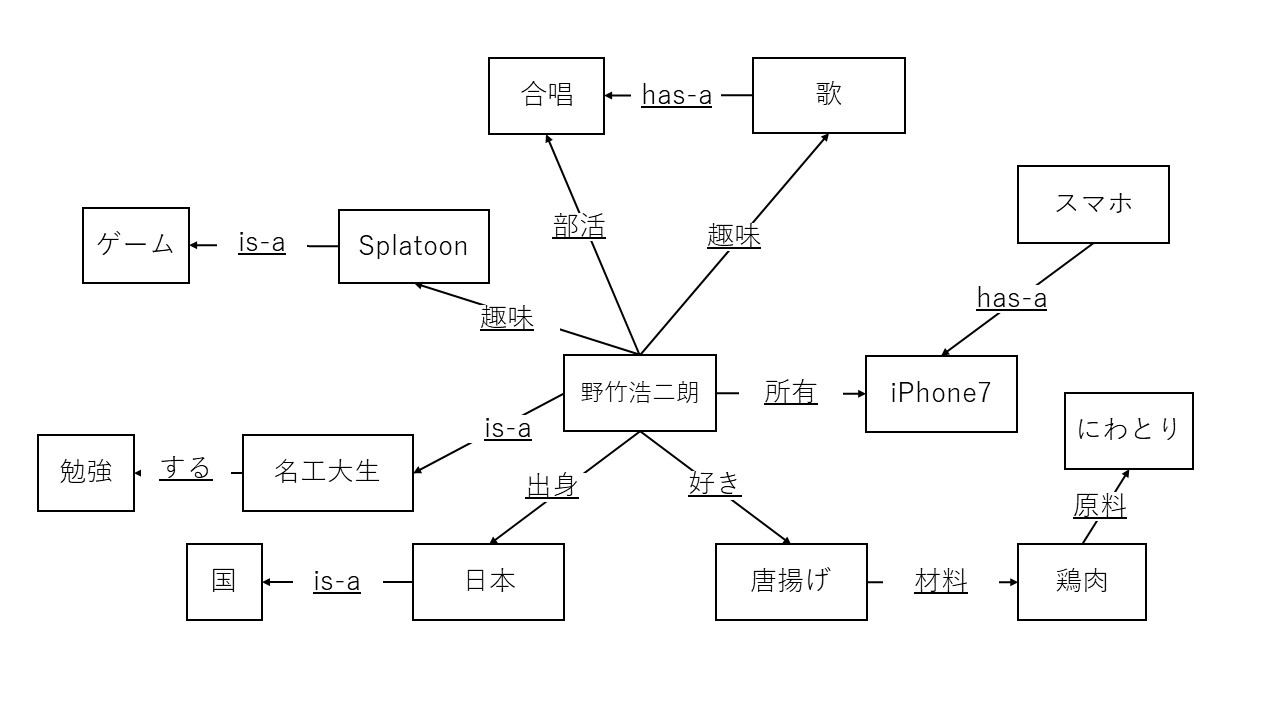
\includegraphics[width=150mm,height=80mm]{Semantic-Kojiro.jpg}

\subsection{実装}
上に示した画像のセマンティックネットをExample.javaを参考に生成する。

\subsection{実行例}
MakeSemanticNet.javaによってセマンティックネットを生成した.その結果を以下に示す.

\begin{screen}
\begin{verbatim}
野竹浩二朗  =is-a=>  名工大生
野竹浩二朗  =趣味=>  Splatoon
野竹浩二朗  =部活=>  合唱
野竹浩二朗  =趣味=>  歌
野竹浩二朗  =所有=>  iPhone7
野竹浩二朗  =好き=>  唐揚げ
野竹浩二朗  =出身=>  日本
名工大生  =する=>  勉強
( 野竹浩二朗  =する=>  勉強 )
Splatoon  =is-a=>  ゲーム
歌  =has-a=>  合唱
スマホ  =has-a=>  iPhone
唐揚げ  =材料=>  鶏肉
鶏肉  =原料=>  鶏
日本  =is-a=>  国
*** Nodes ***
野竹浩二朗
名工大生
Splatoon
合唱
歌
iPhone7
唐揚げ
日本
勉強
ゲーム
スマホ
iPhone
鶏肉
鶏
国
\end{verbatim}
\end{screen}
この結果により、上に示した画像と同様のセマンティックネットが構築できていることが分かる。
\section{課題3-2}
\begin{screen}
フレームのプログラムを参考に,自分達の興味分野に関する知識をフレームで表現せよ.その分野の知識を表す上で必須となるスロットが何かを考え,クラスフレームを設計すること.
個人レポートには自分が作ったインスタンスフレームのみ(クラスフレームの設計担当者はクラスフレームも)を示し,グループレポートにはクラスフレームおよび全員分のインスタンスフレームを示せ.
\end{screen}

\subsection{手法}
ここでは任天堂の『大乱闘スマッシュブラザーズ』というゲームのキャラクターに関するクラスフレームとインスタンスフレームを構築した.構築したフレームは下図のようなものである.


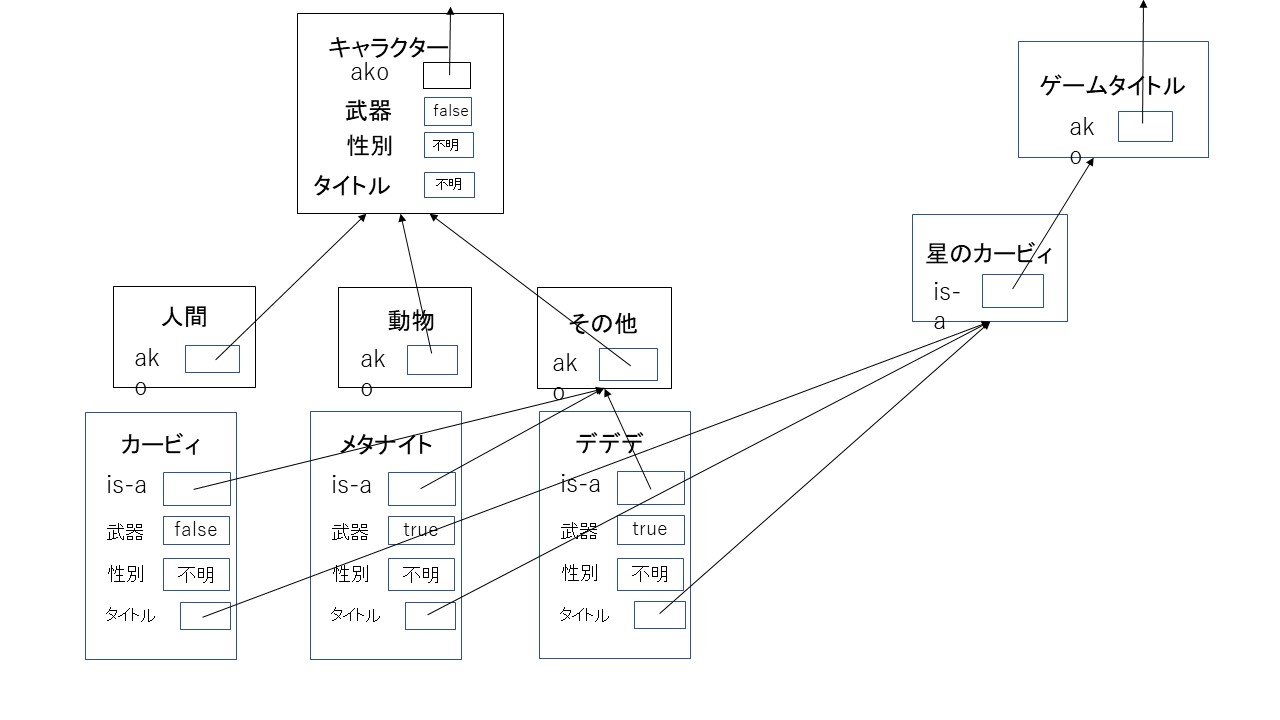
\includegraphics[width=150mm,height=80mm]
{Frame-Kirby.jpg}

この図において「キャラクター」「人間」「動物」「その他」「ゲームタイトル」フレームをクラスフレーム、それ以外をインスタンスフレームとして構築している。


\subsection{実装}
上に示したフレームを生成する.フレームの生成はExample.javaを元に実装した.\\
実装する上で、ゲームタイトルを加えなければならないため、AIFrameSystem.javaとAIFrame.javaにゲームタイトルを格納するフレームを格納する、取り出すメソッドを加えた。
\subsection{実行例}
実際にフレームに格納されている値を表示するメソッドを作り、格納されている値を確かめた。次にその1例を示す
\\

\begin{screen}
\begin{verbatim}
Frame:カービィ
武器:false
性別:不明
タイトル:星のカービィ
\end{verbatim}
\end{screen}
他のキャラクターの値も確かめ、示した図と同じフレームを確認することができた。

\subsection{考察}
今回の課題ではセマンティックネット、フレームの生成をした。\\
セマンティックネットは、お互いに関係のある単語や概念がある時に使える。今回の例で言えば、私の趣味は「野竹浩二朗→Splatoon→ゲーム」とたどることで、直接つながっていなくても趣味がゲームであることが分かる。\\
人が増えたりしてしまうとセマンティックネットが複雑になってしまい、ネットワークが肥大してしまう。それを防ぐためにフレームを設定しネットワークの肥大化を制限するというのが課題3-2であった。\\
セマンティックネットは有向グラフであるため、「ゲームが趣味なのはだれか」というように、グラフの向きと質問における向きが合っていない場合、セマンティックネットを無向グラフのように見なければならず、このネットワークである意味がなくなってしまう。\\
\section{感想}
\end{document}